\documentclass{article}

% if you need to pass options to natbib, use, e.g.:
% \PassOptionsToPackage{numbers, compress}{natbib}
% before loading nips_2018

% ready for submission
%\usepackage{nips_2018}

% to compile a preprint version, e.g., for submission to arXiv, add
% add the [preprint] option:
\usepackage[preprint]{nips_2018}

% to compile a camera-ready version, add the [final] option, e.g.:
% \usepackage[final]{nips_2018}

% to avoid loading the natbib package, add option nonatbib:
% \usepackage[nonatbib]{nips_2018}

\usepackage[utf8]{inputenc} % allow utf-8 input
\usepackage[T1]{fontenc}    % use 8-bit T1 fonts
\usepackage{hyperref}       % hyperlinks
\usepackage{url}            % simple URL typesetting
\usepackage{booktabs}       % professional-quality tables
\usepackage{amsfonts}       % blackboard math symbols
\usepackage{nicefrac}       % compact symbols for 1/2, etc.
\usepackage{microtype}      % microtypography
\usepackage{graphicx}       % include graphics

\title{Analysis of Generating Isolated Tracks from NES Music}

% The \author macro works with any number of authors. There are two
% commands used to separate the names and addresses of multiple
% authors: \And and \AND.
%
% Using \And between authors leaves it to LaTeX to determine where to
% break the lines. Using \AND forces a line break at that point. So,
% if LaTeX puts 3 of 4 authors names on the first line, and the last
% on the second line, try using \AND instead of \And before the third
% author name.

\author{
  Bryan Learn\\
  blearn@andrew.cmu.edu\\
  Carnegie Mellon University\\
  Pittsburgh, PA 15213\\
  \And
  Mike Tasota\\
  tasota@andrew.cmu.edu\\
  Carnegie Mellon University\\
  Pittsburgh, PA 15213\\
}

\begin{document}
% \nipsfinalcopy is no longer used

\maketitle


\begin{abstract}
  % TODO add real abstract text
  A brief overview of our project.
\end{abstract}


\section{Introduction}

% TODO taken from Proposal, revise text
% - What are you trying to solve
% - Why is it important?
% - It should have a thorough and clear explanation of what’s at stake, and in a well-formulated (e.g. mathematically) format

Although similar to text generation in many respects, there is still significant progress to be made in the area of music generation. There are a few distinctions between the problem of music generation and text generation that affect this. The number of potential states that a standard 88-key piano can take greatly exceeds the number of words in any language. Another difference that is present in music generation is the concept of tempo, which adds even more complexity to the number of representations that generated music can take in comparison to generated text.

Previous rule-based models of generation are now being outperformed thanks to the advent of deep learning techniques. One research effort that has made significant progress is the Magenta research project, which was started by researchers and engineers from the Google Brain team. This package utilizes the TensorFlow library to implement various deep learning techniques for the problem of music generation.


\section{Related Work}

% TODO taken from Proposal, revise text

In the MidiNet paper, Yang et al. created a CNN-GAN based model for MIDI generation [4]. They propose that their model could be possibly expanded to generate multiple tracks. This was demonstrated in the work done by MuseGAN. However, as pointed out in the MusicVAE paper, MuseGAN works with a fixed set of instruments, namely bass, drums, guitar, piano, and strings [3]. Instead, MusicVAE is capable of modeling exactly three broad classes of instruments which it calls the “trio:” melody, bass, and drums. This provides more flexibility on what instruments can be assigned in track generation. However, it also introduces chord conditioning to keep harmony fixed.

Another related work in multiple track generation is from Chu et al. in their “Song from PI” RNN. Although PI is capable of producing multiple tracks, they also conditioned the generation on scale types to help pick up regularities in their dataset of pop songs [1]. In our work, we hope to produce multiple tracks without relying on prior knowledge of music theory in the model.


\section{Dataset}

The suggested input data for the music generation project topic was classical piano music pieces from the website www.piano-midi.de. We ultimately decided against this dataset because of its lack of well-defined tracks and sparse variety of instrument voices across all MIDI files. On top of this, the classical piano dataset was relatively small (less than 1,000 MIDI files).

% TODO segue?

% TODO taken from Poster, revise text
For our work, it was necessary to have access to a dataset of MIDI files which had consistent track types across the entire dataset. To accomplish this, we used the NES Music Database (NES-MDB) as presented by Donahue et al. [2]. The dataset consists of 5,278 songs from the soundtracks of 397 NES games. Each MIDI file consists of four instrument voices, each mapping to an NES synthesizer. These voices are two pulse-wave generators (P1, P2), a triangle-wave generator (TR), and a percussive noise generator (NO). Since these voices are consistent throughout all files in the dataset, we assumed that each voice represented a specific track type. For example, the percussive noise generator would be a drum track for all MIDI files in which it is defined.

% TODO mention other artifacts in MIDI files that are being ignored (all the Control_c events)


\section{Methods}

% - describe what work you have completed towards creating a method or pipeline which improves on the baseline.
% - What is your motivation behind these techniques
%   --(you are highly encouraged to come up with an original idea of your own rather than simply implementing or applying an existing ML algorithm)
% - Use math/figure to explain your approach, when possible (do not use a lot of space on page)

% TODO taken from Poster, revise text
To train on specific voices, we modified the original MIDI dataset to generate four single-track datasets for each of the four tracks present (P1, P2, TR, NO). This was achieved using the midicsv and csvmidi tools developed by John Walker. By converting the MIDI files to CSV format, we were able to automate the process of extracting single tracks from each file in the dataset. Then we passed each of the modified single-track datasets through the MelodyRNN and MusicVAE pipeline. For both MelodyRNN and MusicVAE, the first step is to build a note sequences (.tfrecord) file which can be read in by most of the Magenta models. It is also worth noting that the isolated drums track (NO) had to be modified further to properly train on the MelodyRNN model. As per the General MIDI standard, the channel specified by NO (channel 9) was dedicated to percussion, and the first step taken by MelodyRNN was to remove this track. To resolve this, we simply modified our script for NO to also modify the track’s MIDI channel.


\section{Experiments}

% - Show plots of the performance of your algorithms and interpret what they mean
%   --Be sure to label and explain this clearly
% - What do the results imply about your methods?

Since our interests lie in learning individual voice classes, we used models trained on the original dataset as well as models trained on the four individual voice classes (P1, P2, TR, and NO). This allowed us to audibly compare differences in what the baseline model learned to what our voice-specific models learned. Also, for RNN, we compared our isolated track models to the baseline model from their calculated training losses.

\subsection{Training the Baseline}
We wanted a baseline comparison for the two Magenta models that we considered (MusicVAE and MelodyRNN). To accomplish this, we trained with the original NES-MDB Dataset with all four voices. For the MusicVAE baseline we used the Trio configuration, where “trio” refers to an ensemble of three performers or voices. MusicVAE’s trio consists of melody, bass, and drums, and it uses chord conditioning to keep harmony fixed. We also trained the MelodyRNN baseline model, but the MelodyRNN configuration only produces one melody in contrast to the trio.

\subsection{Isolated Track Training}
We trained both the MusicVAE model and the MelodyRNN model on each of the four isolated tracks for a total of 8 track-separated models. The models were trained on the Bridges environment provided by the Pittsburgh Supercomputing Center using a mixture of regular memory nodes and GPU nodes. Each model was trained up to 8 hours. The MelodyRNN models that were trained for 8 hours were overfitting. To address this we compared the performance of earlier versions of the models to the overfit models by evaluating test loss.

When training drums for MelodyRNN, we learned that the basic MelodyRNN configuration ignored all information from the MIDI channel associated with percussion. For learning drums, a separate model exists in the project (DrumsRNN). However, our training indicated that training percussion on DrumsRNN only produced one note value despite having multiple percussive note values in the training data. We successfully preserved this information in the training by modifying the MIDI files in our NO dataset to use a non-percussive MIDI channel and training with MelodyRNN.

% TODO mention/include figure comparing DrumRNN, MeodyRNN
\begin{figure}[htb!]
  \begin{minipage}{0.48\textwidth}
    \centering
    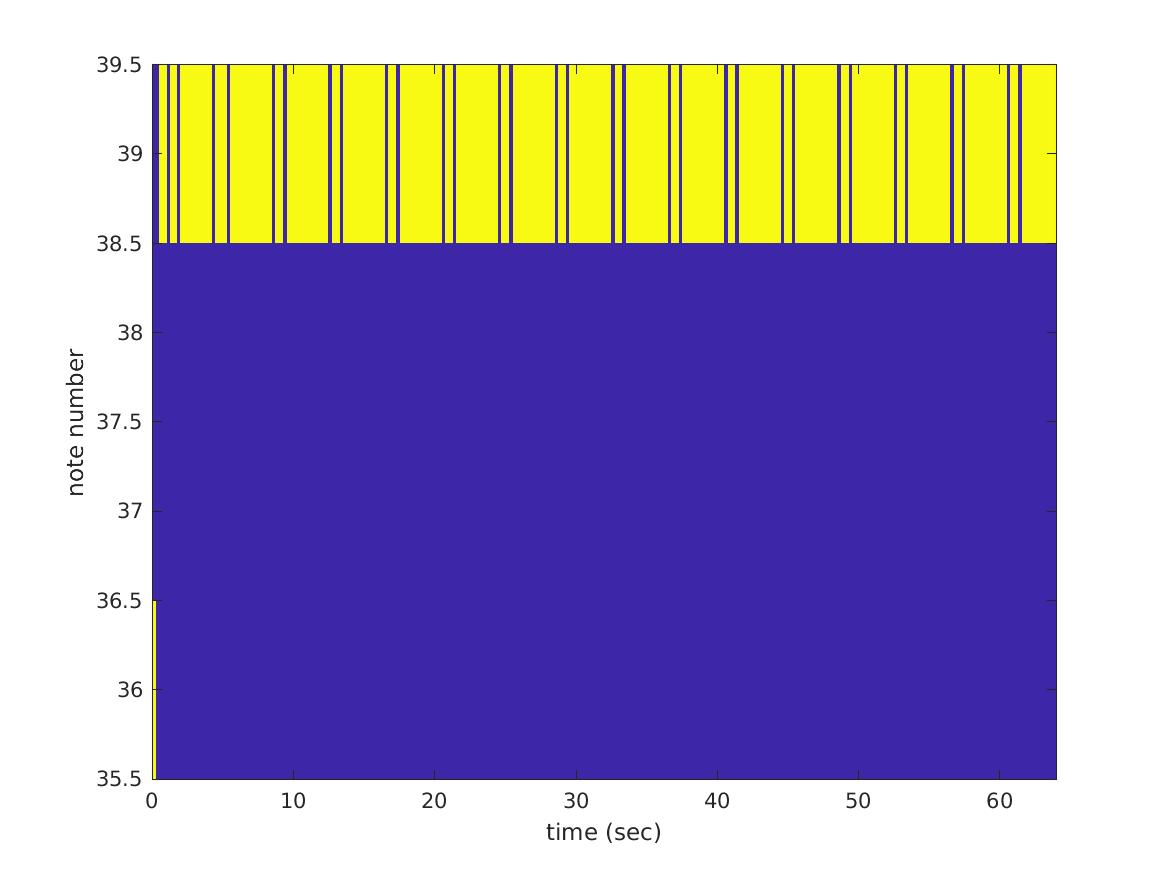
\includegraphics[height=4cm, width=4cm]{img/DrumRNN_drum.jpg}
    \caption{DrumRNN: percussive track}
  \end{minipage}\hfill
  \begin{minipage}{0.48\textwidth}
    \centering
    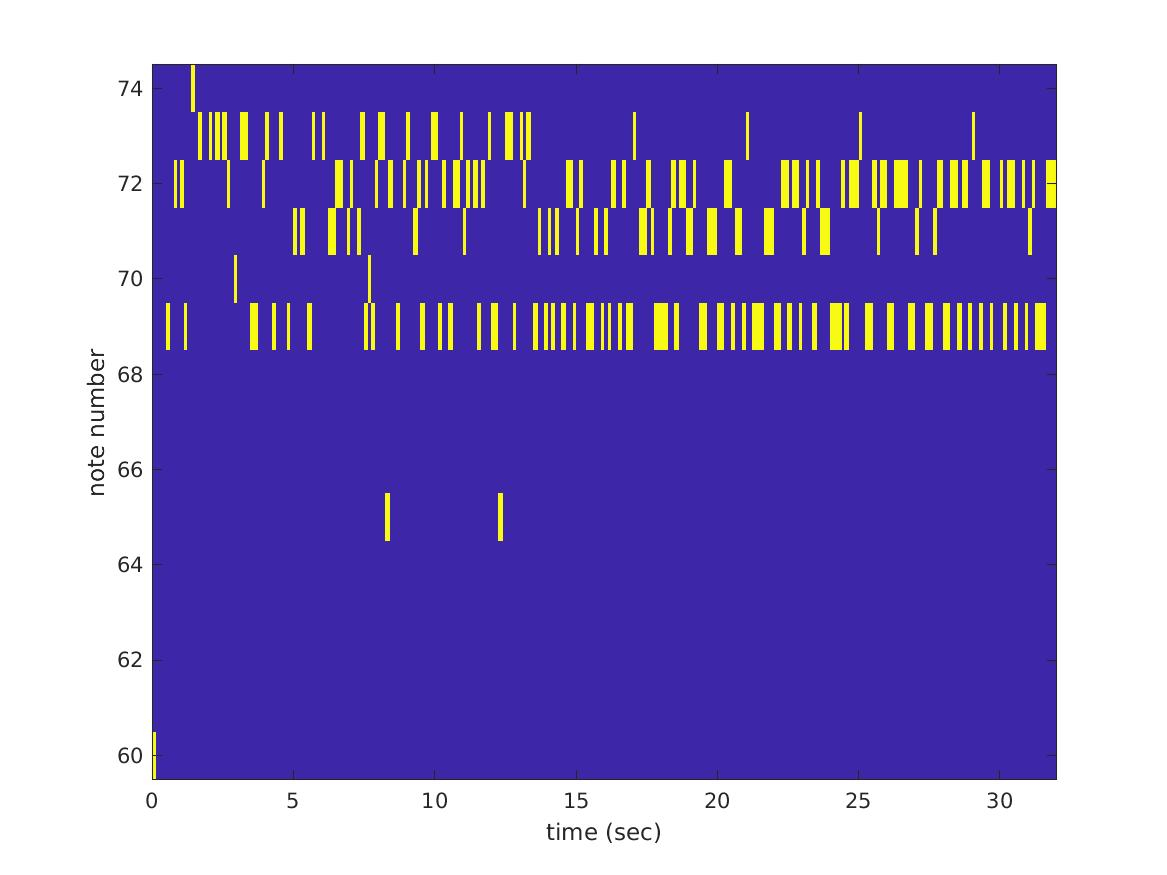
\includegraphics[height=4cm, width=4cm]{img/MelodyRNN_drum.jpg}
    \caption{MelodyRNN: percussive track}
  \end{minipage}
\end{figure}

\subsection{Generated Tracks}
After generating the isolated tracks, we were interested in converting the generated MIDI files into synthesized NES tracks. As part of the NES-MDB project, there is a tool for converting MIDI files from the dataset into audio files generated from synthesized track voices. However, we learned that the generated format from the models was not enough to generate synthesized voices. This is because the original dataset included control event information to produce more expressive voices, and this information was not generated as output from our models.


\section{Results}

We evaluated the trained models by listening to the generated music and comparing the training loss across model types. For MelodyRNN, the training loss trend for each isolated track was less than the training loss for the baseline model. The graph for training loss in the MusicVAE model only includes models which trained beyond the initial checkpoint (P1, P2, TR). When considering the number of isolated tracks that were learned, the RNN models outperform the VAE models. The MusicVAE baseline and percussive track (NO) never went beyond the initial checkpoint in its training. This resulted in the models generating mostly random noise <INCLUDE FIGURE OF WHITE CHRISTMAS>. For MusicVAE, it is interesting that training never went beyond the initial checkpoint for all training data that included percussion. Even when modifying the files to use a non-percussive MIDI channel type, the MusicVAE model failed to train beyond its initial checkpoint.

% TODO add figure for reference to MusicVAE White Christmas
\begin{figure}[htb!]
  \begin{minipage}{1.0\textwidth}
    \centering
    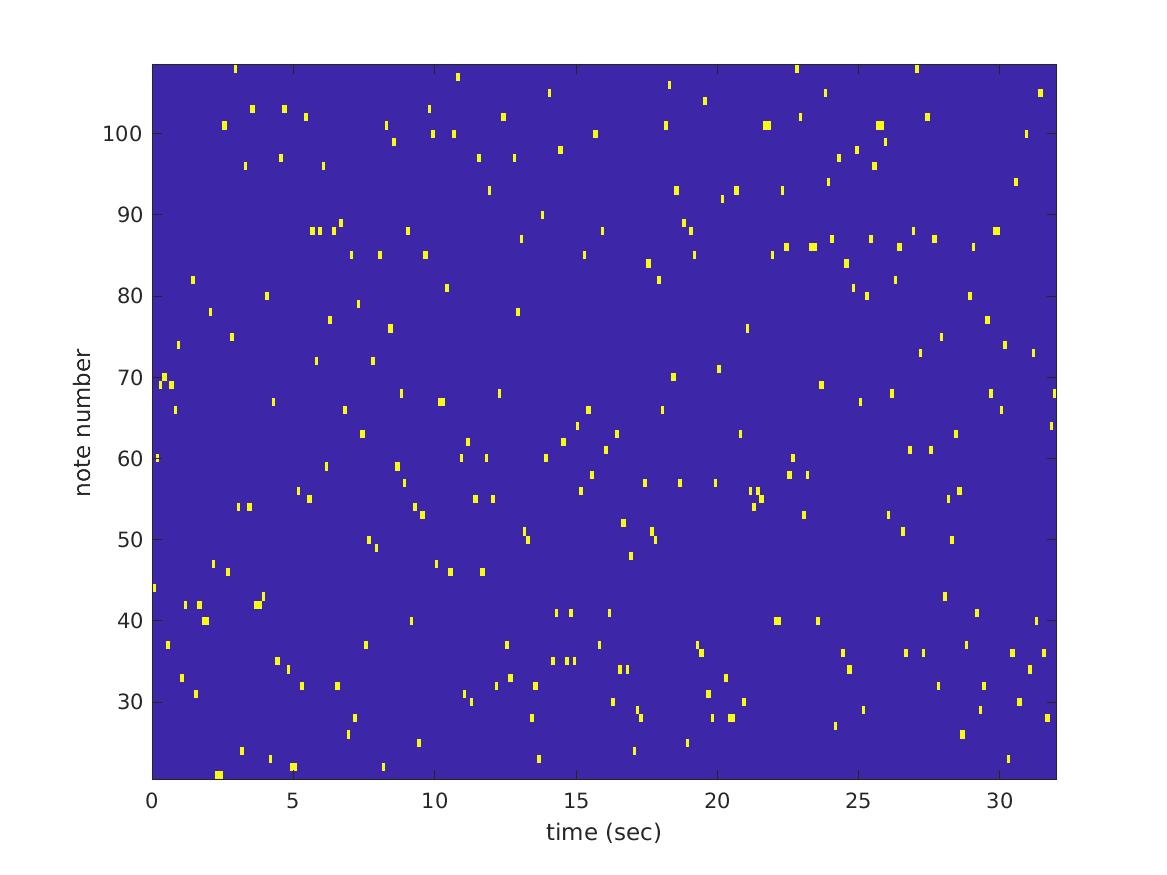
\includegraphics[height=4cm, width=4cm]{img/vae_no.jpg}
    \caption{MusicVAE: percussive track}
  \end{minipage}
\end{figure}

An additional evaluation on the generated music indicated that the RNN models produced better results than the VAE models. These results were surprising as our preliminary results seemed to indicate that the MusicVAE model was capable of generating more interesting melodies. This prior analysis was based on pre-trained models provided by the Magenta project, and the data which produced these pre-trained models is not documented. The shortcomings of the results of the VAE models could possibly be the result of a lack of data or allocated time for training.

% TODO We will definitely want to reference the musicVAE paper where they explain they used ~1.5midi files to train
% TODO might want to explain why VAE has less checkpoints


\section{Conclusion and Future Work}

% TODO add conclusion

% - what you accomplished and what would be the future direction for this project
% - Analyze your model and results
% - Highlight a few limitations of your approach (assumptions made, pitfalls, caveats, etc.)
% - Comment on whether you think there is a way to further improve your method to eliminate these limitations

\section{Acknowledgements}
We thank our project mentor, Jing Mao, for assistance.\\

This work used the Bridges system, which is supported by NSF award number ACI-1445606, at the Pittsburgh Supercomputing Center (PSC).

\section*{References}

% TODO needs updated for final report references

\small

[1] Chu, Hang, et al. ``Song From PI: A Musically Plausible Network for Pop Music Generation.'' {\it [1611.03477] Song From PI: A Musically Plausible Network for Pop Music Generation,} 10 Nov. 2016, arxiv.org/abs/1611.03477.

[2] Donahue, Chris et al. ``The NES Music Database: A multi-instrumental dataset with expressive performance attributes'' {\it [1806.04278] The NES Music Database: A multi-instrumental dataset with expressive performance attributes,} 12 June 2018, arxiv.org/abs/1806.04278.

[3] Simon, Ian, et al. ``Learning a Latent Space of Multitrack Measures.'' {\it[1806.00195] Learning a Latent Space of Multitrack Measures,} 1 June 2018, arxiv.org/abs/1806.00195.

[4] Yang, Li-Chia, et al. ``MidiNet: A Convolutional Generative Adversarial Network for Symbolic-Domain Music Generation.'' {\it[1703.10847] MidiNet: A Convolutional Generative Adversarial Network for Symbolic-Domain Music Generation,} 18 July 2017, arxiv.org/abs/1703.10847.

\end{document}
